% =====================================================================
%  G2 - Per-candidate tally time vs candidate count (n=1000)
%  --------------------------------------------------------------------
%  Backs the claim: O(1) per candidate, candidate-independent scaling
%  Source: chapter4.tex Table tab:candidate-scale
% =====================================================================
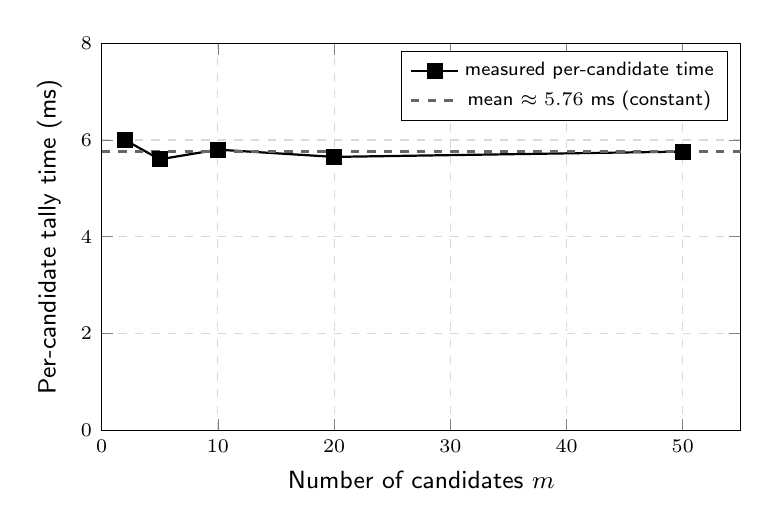
\begin{tikzpicture}
\begin{axis}[
    width=0.80\textwidth,
    height=6.5cm,
    xlabel={Number of candidates $m$},
    ylabel={Per-candidate tally time (ms)},
    ymin=0, ymax=8,
    xmin=0, xmax=55,
    grid=both,
    grid style={dashed, gray!30},
    legend style={at={(0.98,0.98)}, anchor=north east,
                  font=\sffamily\scriptsize, draw=black},
    label style={font=\sffamily\small},
    tick label style={font=\sffamily\scriptsize},
    every axis plot/.append style={thick},
]
% Per-candidate time from Table tab:candidate-scale (n=1000)
\addplot+[mark=square*, mark size=2.5pt, color=black, mark options={fill=black}] coordinates {
    (2,  6.00)
    (5,  5.60)
    (10, 5.80)
    (20, 5.65)
    (50, 5.76)
};
\addlegendentry{measured per-candidate time}
% Constant reference at ~5.76 ms (mean)
\addplot[domain=0:55, samples=2, dashed, thick, color=black!60] {5.76};
\addlegendentry{mean $\approx 5.76$ ms (constant)}
\end{axis}
\end{tikzpicture}
